\begin{minipage}[t]{180mm}
\fcolorbox{black}{white}{
\begin{minipage}[b]{30mm}

\includegraphics[width=0.5\linewidth]{unflogo.pdf}
\end{minipage}
\begin{minipage}[b]{100mm}
\Huge \textbf{UNF NEWZ} \\
\Large -- Søvn og retsstavning er overvurderet! 
\end{minipage}
\begin{minipage}[b]{50mm}
\Large Onsdag 17.07.2015 \\
\normalsize Redigeret i \LaTeX\ af \\ SOM, MGS, MMN, SABH
\end{minipage}
}
\end{minipage}



\begin{minipage}[b]{0.95\linewidth}
\begin{minipage}[t]{0.47\textwidth}
\vspace{3mm}
\section*{Koordinativ Resolution}

Paa Campens derom nedlagte allerunderdanigste Forestilling har det under den femtende i Ormemaaneden i det tohundredeseksogtredivte Aar behaget mig, Campens Koordinator af Gauss' Naade, Eulers Husholder og Galois' ydmyge Efterfølger, at afstaa al Eierskab af Husalfen i en begrænset Periode mellem Solopgang og Solnedgang denne femtende i Ormemaaneden i det tohundredeseksogtredivte Aar. Dette vil dog ingenlunde begrænse Husalfens Forpligtelser, hverken over for Campen eller over for dens Tjenestemænd. Under mit Eierskabs Fravær paalægges Ansvaret for Tilsynet over Husalfens Ve, Vel og Opførsel det til dette Formaal nedsatte Konsistorium, bestaaende af de Arrangører paa Campen hvis upaaklagelige Ry gør dem egnet til Hvervet. Exekutivt opretholdes den Gaussgivne orden af de dertil udpegede Campforstandere som udpeges fra de ikke-svenske af Landets enkeltsammenhængende Provinser og som for at dokumentere deres Representationsret forventes offentligt at anerkende deres Tilhørsforhold til Drøvtyggernes Loge, og samtidigt sværge deres afstandstagen fra Ordinatorens magtfuldkommenhed.

{\flushright\emph{Morten Grue Sørensen, Koordinator af Gauss' Naade }}

\section*{Deltagere eller Rotter?}
Det er blevet bragt til UNF Newz redaktionen opmærksomhed at der fra AUs side var planer om at der i Aud E. i perioden fra torsdag den 11. og 2 uger frem skulle dekonterminernes for rotter! Dette ville have involveret stører mængde gas, adskillige fælder og mænd i fuld ABC-Dragt \footnote{ Atomare / Nucleare, Biologiske og kemiske(Chemical) substanser}.  Om AU har været bevist om at der realt set var Matematik Camp i denne periode er ikke UNF Newz bekendt, men noget tyder på at AU havde hørt om Mat-Camp. Antagelsen at AU viste om Mat-Camp leder til det simple spørgsmål om deltagere, i AUs øjne, er rotter?
Og vil de komme i løbet af ugen for at udrydde dem? \\
Efter at disse spørgsmål er blevet stillet at UNF Newz banebrydende journalistik har Mat-Camps ledelse i gang sat en stører undersøgelse af hvorvidt de skal støtte op om Camps hoved sponsor i udryddelsen af AUs nye skadedyr.

\vspace{2mm}
{\centering
\includegraphics[width=\textwidth]{Rats.jpg}
}

\end{minipage}
\hfill\begin{minipage}[t]{0.47\textwidth}

\vspace{1mm}
\tikzstyle{mybox} = [draw=white, fill=blue!20, very thick,
    rectangle, rounded corners, inner sep=10pt, inner ysep=20pt]
\tikzstyle{fancytitle} =[fill=red, text=white]

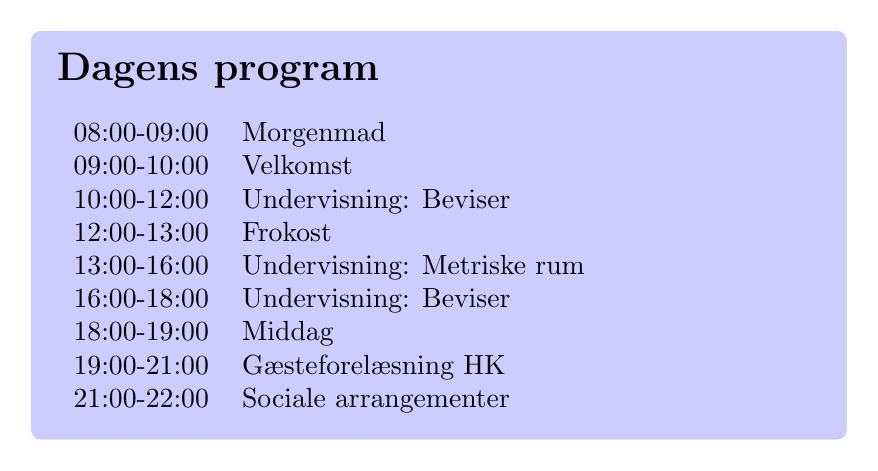
\begin{tikzpicture}
\node [mybox] (box){%
\begin{minipage}{0.80\textwidth}
\vspace{-4mm}\section*{Dagens program}
\begin{tabular}{ll}
08:00-09:00 & Morgenmad \\
09:00-10:00 & Velkomst \\
10:00-12:00 & Undervisning: Beviser \\
12:00-13:00 & Frokost \\
13:00-16:00 & Undervisning: Metriske rum \\
16:00-18:00 & Undervisning: Beviser \\
18:00-19:00 & Middag \\
19:00-21:00 & Gæsteforelæsning HK \\
21:00-22:00 & Sociale arrangementer
\end{tabular}
\vspace{-4mm}
\end{minipage}
};
\end{tikzpicture}%

\section*{Produktanmeldelse -- A2-printer}
Ved andet øjekast ses straks at hér var der alligevel ikke kræset for detaljerne. Printeren burde være ansvarlig for at printe al det fantastiske faglige materiale, men selv denne anmeldelse af A2-printeren har den bestemt sig for ikke at udskrive. Der findes på IMF også en A3- og A4-printer, og som navnene antyder, er de særdeles mere funktionelle end krøblingen A2. Selvom den hedder A2, indeholder printeren ikke A2-papir -- det største er A3-papir, hvilket i forvejen udskrives glimrende fra A3. Den foldning og hæftning af hæfter som A2 har udført inden den afgik ved døden har desuden ikke samme flair og udstråling som de med møje håndsamlede sanghæfter konstrueret med assistance fra ``the Clipsemaskine of Doom''.
Med sine knebne 0 sider per minut, er A2 i realiteten komplet ubrugelig for alle matematikere uanset antallet af dimensioner disse måtte befinde sig i. A2-printerens blanke matte design og grålige nuance giver en så frastødende discount-udstråling at printeren ikke bør gives til børn under 3 år eller noget andet individ. Det rapportes desuden at UNF Newz-redaktionens udsendte medarbejder besvimede af sensorisk overbelastning og måtte reddes væk ved hjælp reb affyret med bue og pil fra sikker afstand. Korrespondentens tilstand rapportes her til aften at være stabil og uden for livsfare. UNF Newz udtrykker i denne sammenhæng stor tak til ABR for hurtige og præcise bueskud i forbindelse med redningsaktionen.

\vspace{1mm}
\section*{Madanmeldelse -- Uni-pizza pizza}
\fcolorbox{black}{white}{$1$ ud af $\aleph_1$ chokoladekiks}

\vspace{2mm}

Med glæde så vi frem til denne midtjydske specialitet, som vi huskede fra 2009 og 2011. Desværre blev vi kort efter modtagelsen dybt skuffede, hovedingrediensen var blevet fjernet, og vi blev overmandet af savnet. Pomfritter var der ingen af på denne pizza, meget skuffende, når man nu havde set frem til dem i to år, og af rent afsagn levet af portvin og sushi. AU uden pomfritpizza er jo som Sverige uden surstrømning eller Færøerne uden mugne fårehoveder, mindre afstødende, men uden kulturel identitet, og derfor bare en billig kopi af brokvarterenes baggårde  og deres forhutlede eksistenser, som segner hen i rødbedemisbrug og livslange bachelorstudier på KUA. 

\end{minipage}
\end{minipage}
